\documentclass[titlepage]{article}

\usepackage[margin=1in]{geometry}
% some more shit for the title
\usepackage[T1]{fontenc}
\usepackage{babel}

% Tables and stopping them from displaying in a different section
\usepackage{booktabs}
\usepackage[section]{placeins}

% for inserting images into the document, setting file path, and allowing rotation of inserted images 
\usepackage{graphicx}
\graphicspath{ {./images/} }
\usepackage{rotating}
\usepackage[table]{xcolor}
% mostly just for putting text in math equations
\usepackage{amsmath}
% for aligning the text to the left
\usepackage[document]{ragged2e}

% for inserting hyperlinks in the document, use \url{url} or \href{url}{text}
\usepackage{hyperref}
\usepackage{calligra}
\usepackage[T1]{fontenc}
\usepackage{siunitx}
\usepackage{caption}
\usepackage{multirow}
\usepackage[export]{adjustbox}
\usepackage{tikz}
\usepackage{pgfplots}
\pgfplotsset{soldot/.style={color=black,only marks,mark=*},
	             holdot/.style={color=black,fill=white,only marks,mark=*},
		                  compat=1.12}
\usepackage{paracol}

\begin{document}
\title{\textbf{Lab 4: Resistivity of Nickel Chromium Wire and Use of the Wheatstone Bridge Circuit}}
\author{
    Zachary Pouska\\
    \texttt{001103193}\\
    \and
    Natalie Tran \\ 
    \texttt{000698629}\\ \\
    \and
    Joseph Pancho\\
    \texttt{002550975} \\ \\
} 

\date{PHYS 236 | Fall 2022\\
Date performed: 10/10/2022}


	\maketitle



	\section{Purpose}
	In this lab, we measured the resistance of a nickel chromium wire 
	and calculated the resistivity $\rho$. We then built a Wheatstone 
	bridge to find the resistances of individual capacitors.

	\section{Theory}
        \subsection{Part 1} 
	Using nickel chromium wire $(80\%~Ni- 20\%~Cr)$, we will apply the 
	equations for calculating resistivity $\rho$. \\
	~\\
	For a given wire resistivity $\rho$, length $L$, and cross-sectional 
	area $A$, the resistance $R$, is given by: \\
	\[
		R=\frac{\rho L}{A}
	\]
	Solving for $\rho$, the above equation is re-written as:
	\[
		\rho = \frac{RA}{L}
	\]	 
	Verifying the untis for $\rho$: 
	\[
		\rho=\frac{\Omega m^2}{m}=\Omega m	
	\]

    \subsection{Part 2} 
        In a Wheatstone bridge, the wire connecting the two parallel resistors will have a point where the potential is 0 relative to the two pairs of series resistors, or in our case the point between our resistor box and the unknown resistor. In our setup, the nichrome wire is acting as our upper two resistors of a Wheatstone bridge, as it is divided essentially into two resistors. Using this phenomenon, we can "calibrate" the Wheatstone bridge by moving the point of contact across the nichrome wire, which then lets us assume that the points $P_1$ and $P_2$ have equal electric potentials. 


	\section{Experiment Analysis}
        
        \subsection{Measurement of the resistivity $\rho$} 




    In part 1, our objective is to measure the resistivity constant of our nichrome wire. We can use the following equations to calculate the resistivity:
    $$\rho = R \frac{A}{l} \text{ where } A=\pi r^2$$ 
    $$ R=\rho \frac{l}{A} = \rho \frac{l}{\pi r^2}  \text{ in this case, R is a function of $\rho$, $l$, and $r$} $$

    Having used these equations, we found that the resistance of the wire, $R$, was 7.4$\Omega$, and the resistivity of the wire was equal to $(7.4)\frac{\pi \cdot (0.227 \cdot 10^{-3})^2}{1.0m} = 1.199\cdot 10^{-6}$. 

    The \textbf{uncertainty} of our measurement of the resistance was determined using the formula $$\Delta f= \frac{\partial f}{\partial x} \Delta x + \frac{\partial f}{\partial y} \Delta y + \frac{\partial f}{\partial z} \Delta z$$ for a function $f(x,y,z)$.
    Substituting in our values, we obtain the equation:
    $$\Delta R= \frac{\partial R}{\partial \rho} \Delta \rho + \frac{\partial R}{\partial l} \Delta y + \left|\frac{\partial R}{\partial r}\right| \Delta r$$ 
    Where $\partial \rho = \frac{l}{\pi r^2}$, $\Delta \rho = \text{range}$, $\partial l = \frac{\rho}{\pi r^2}$, $\Delta l =\text{resolution of meter stick + standard deviation of measurements}$, $\partial r = \frac{\rho l}{\pi}\cdot \frac{-2}{r^3}$ 
    
    


        \subsection{Part 2} 
        In a Wheatstone bridge, the wire connecting the two parallel resistors will have a point where the potential is 0 relative to the two pairs of series resistors, or in our case the point between our resistor box and the unknown resistor. In our setup, the nichrome wire is acting as our upper two resistors of a Wheatstone bridge, as it is divided essentially into two resistors. Using this phenomenon, we can "calibrate" the Wheatstone bridge by moving the point of contact across the nichrome wire, which then lets us assume that the points $P_1$ and $P_2$ have equal electric potentials. 

        \FloatBarrier
        \begin{figure}[hbt!] 
            \centering 
            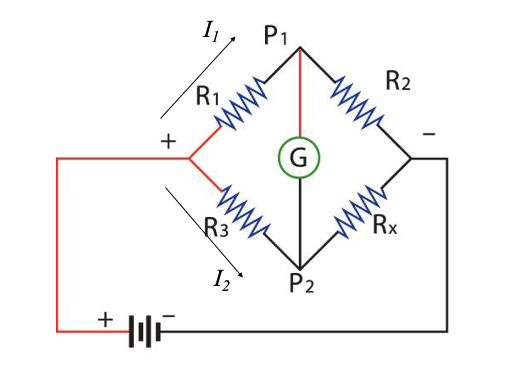
\includegraphics[scale = 0.4]{exanal/wheatstone}
        \end{figure}
        \FloatBarrier

        Then applying Kirchhoff's law from point $P_2$ to point $P_1$ travelling clockwise, we get $$V_{P2}+I_2 R_3 - I_1 R_1  V_{P1} $$ 
        $$ V_{P2} - V_{P1} = I_1 R_1 - I_2 R_3 $$
        and $$ I_1 R_1 = I_2 R_3$$
        Then traveling counter-clockwise, we get $$V_{P2}-I_2 R_x + I_1 R_2 = V_{P1} $$
        $$ V_{P2} - V_{P1} = I_2 R_x - I_1 R_2 = 0V $$
        $$I_2 R_x = I_1 R_2 $$
        and $$\frac{R_1}{R_2} = \frac{R_3}{R_x} $$ which can be further solved for $R_x$, giving us 
        $$R_x = \frac{R_s R_2}{R_1} $$
        where $R_s$ is our known standard resistor box. 

        Substituting our proportional values for $R_1$ and $R_2$ gives us $$R_x = \frac{R_s \left( \frac{\rho L_2}{A} \right)}{\left( \frac{\rho L_1}{A}  \right)} $$ But can still be further simplified to $$R_x=\frac{R_s L_2}{L_1} $$
since the values of the resistances are directly proportional to the lengths of each side of the wire (all other variables like the area and resistivity are held constant). 





	\section{Procedure}
	For the first part of the lab, we first took six measurments of diameter 
	of the nichrome wire (mounted on a bridge-board) using calipers, two measurments per group member.
	Using the data, we then calculated cross-sectional area of the wire ($\pi r^2$) and resistivity 
	($\rho = \frac{RA}{L}$), where $R$ is the resistance ($\Omega$) of the wire measured with a 
	digital multimeter, $A$ is the cross-sectional area, and $l$ is the length of the wire.  
	The resistivity we found was compared to the given range of resistivity of a 
	nichrome wire: ($1.10*10^{-6}~\Omega m~to~1.50*10^{-6}~\Omega m$). \\
	~\\  
	For the second part of the lab, we put together a wheatstone bridge circuit using 
	the nichrome wire bridge-board, a power supply, a digital multimeter, a decade 
	resistance box, six unique resistors (tested one at a time), and alligator clips.
	A diagram of the circuit is shown below: 

	\begin{center}
		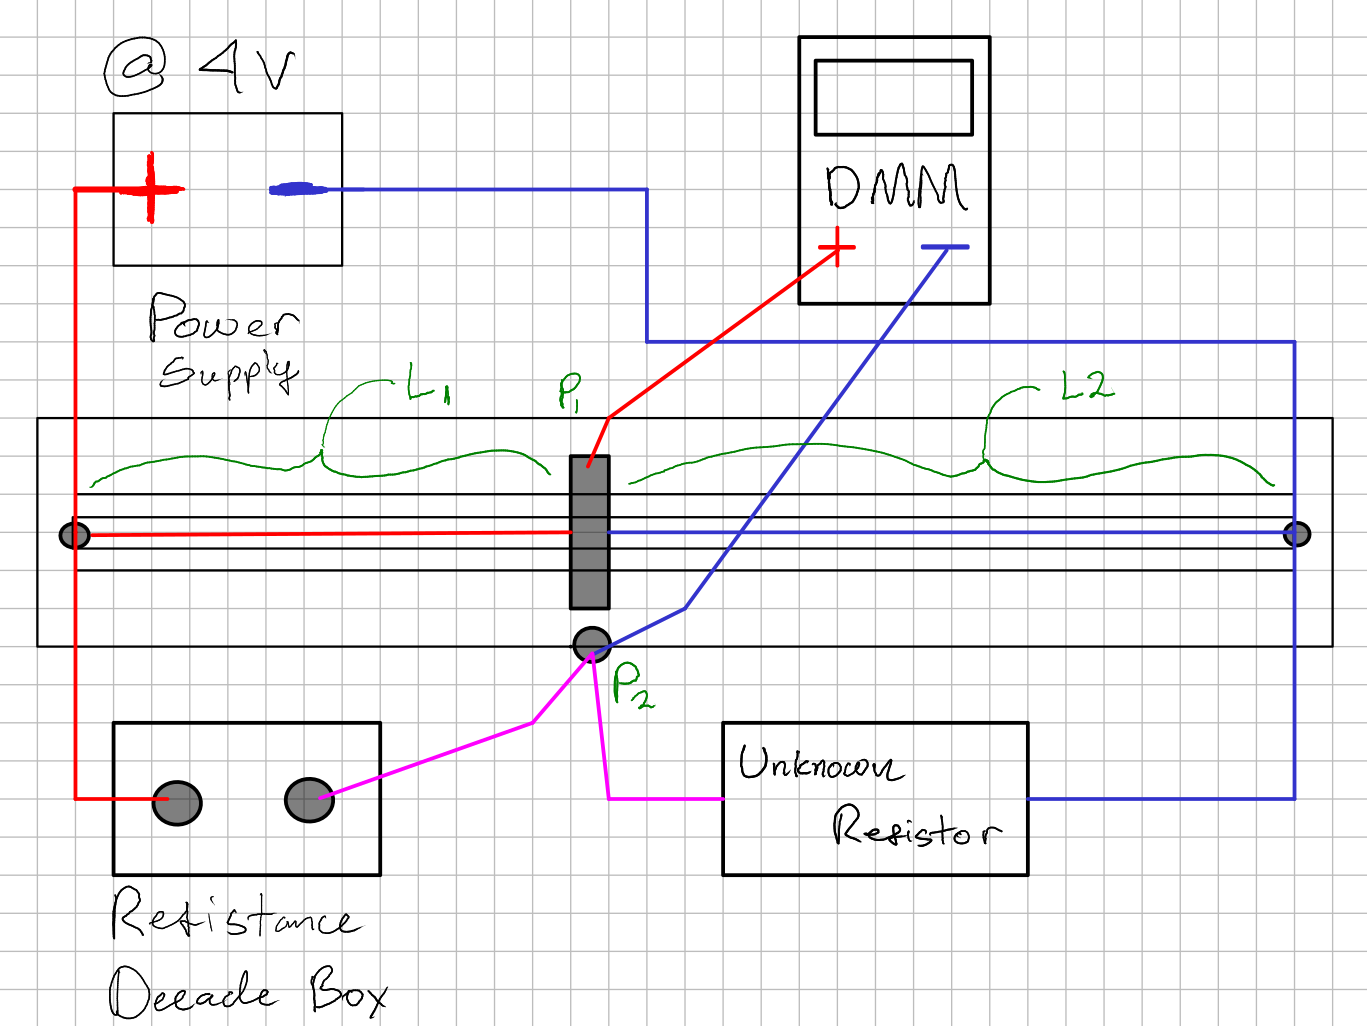
\includegraphics[scale=.2]{lab-circuit-diagram.png}
	\end{center}

	The digital multimeter's ground probe is afixed to a conductive screw on the edge of the 
	bridge-board $P_2$. The positive probe of the multimeter is free to move along the length 
	of the wire to find the where $V=0$, giving us lengths $L_1$ and $L_2$. Since the 
	resistances of the decade box and the unknown resistor are proportional to $L_1$ and $L_2$
	respectively, we can find the the value of the unknown resistance using:
	\[
		R_u=\frac{R_k L_2}{L_1}	
	\]
	Where $R_u$ is the unknown resistance and $R_k$ is the known resistance of the decade box. 
	

	\section{Data and Graphs}
	\subsection{Measurement of the resistivity $\rho$}
	\begin{table}[ht]
		\caption*{[Table 5.1.1] Measurements of the Nichrome wire's diameter.}
		\begin{center}
		\rowcolors{2}{gray!10}{gray!40}
		\begin{tabular}{c|c|c}
			Lab Partner & Diameter(cm) & Radius(cm) \\
			\hline
		        \cellcolor{white}		    &0.05  &0.025 \\
			\cellcolor{white}\multirow{-2}{*}{Natalie} & 0.0445 & 0.2225 \\
			\hline
			\cellcolor{white} &0.045 &0.0225 \\
			\cellcolor{white}\multirow{-2}{*}{Joseph} &0.44 &0.022 \\
			\hline
			\cellcolor{white} &0.0435 &0.02175 \\
			\cellcolor{white}\multirow{-2}{*}{Zach} &0.0459 &0.02295\\
			\hline
			\multicolumn{2}{|c|}{\cellcolor[HTML]{FFFFFF}{Average}} & 0.0227 \\
			\hline
			\multicolumn{2}{|c|}{\cellcolor[HTML]{FFFFFF}{Standard Deviation}} & 0.00118\\
			\hline
		\end{tabular}
	\end{center}
\end{table}
\begin{center}
	\textbf{Calculated cross-sectional area of wire}:
	$$A = \pi r^{2} = 161.88 nm^{3}$$\\
	\textbf{Measured Resistance of the wire}:
	$$R = 7.4\Omega$$
	\textbf{Calculated experimental value of resistivity}:
	$$\rho = 1.1988\cdot 10^{-6}  \Omega m$$
	\textbf{Upper percent error}: 
	$$20.08\%$$
	\textbf{Lower percent error}:
	$$8.98\%$$
	\textbf{Calculated value of the wire conductivity}:
	$$\sigma = 834\cdot 10^{3} \frac{1}{\Omega m}$$
	\textbf{Uncertainty of the calculated resistance}
	$$\Delta R = 9.77\Omega$$
	$$7.4 \pm 9.77$$
\end{center}
	\subsection{Wheatstone Bridge} 
	\begin{table}[ht]
		\begin{center}
			\caption*{[Table 5.2.1] Finding the resistance of an unknown resistor using the wheatstone bridge.}
			\rowcolors{2}{gray!10}{gray!40}
		\begin{tabular}{c|c|c|c|c|c|c}
			Unknown Resistor & R($\Omega$) & $L_1$ & $L_2$ & $R_x$ & DMM $R_x$ & Percent Difference \\
			\hline
			$R_{1x}$ & 610 & 0.927 & 0.073 & 48.0 & 52.6 & 8.68\\
			$R_{2x}$ & 610 & 0.641 & 0.359 & 341.6 & 346.2 & 1.32\\
			$R_{3x}$ & 1610 & 0.417&0.583& 2251& 2241& 0.44\\
			$R_{4x}$ & 20010 &0.438&0.562& 25675&25760&0.33\\
			$R_{5x}$ & 600010 &0.482&0.518& 644824&645000&0.03\\
			$R_{6x}$ & 1000010 &0.128&0.872& 6812568&6800000&0.18\\
		\end{tabular}
	\end{center}
	\end{table}
	\section{Calculations and Results}
	The following is a list of equations used for each experiment section. All results are included in the tables under section 5.
	\subsection{Measurement of the resistivity $\rho$}
	To measure resistivity $\rho$, recall the equation:
	$$R = \frac{\rho L}{A}$$
	Which can be rewritten as:
	$$\rho = \frac{RA}{L}$$
	thus resistance, cross-sectional area, and length of the nichrome wire must be found. \\
	\vspace{0.5cm}
	The cross-sectional area of a circular wire can be found with the expression:
	$$A = \pi r^{2}$$
	\vspace{0.5cm}
	The resistance over the length of the wire was measured using a digital multi-meter.\\
	\vspace{0.05cm}
	The length of the wire that the resistance is being measured over can be found using an observable measuring contraption, such as a meter stick.\\
	\vspace{0.5cm}
	Then to measure the percent error, the utilized expression is:
	$$\text{Percent Error} = \frac{|\text{experimental} -\text{ theoretical}|}{-\text{theoretical}} \times 100$$
	To calculate the upper percent error, the higher theoretical threshold is used, whereas the lower one is used for the lower percent error.\\
	The calculation of the conductiviy of the wire is:
	$$\sigma = \frac{1}{\rho}$$
	To find the uncertainty of the resistance, the given equation is:
	$$\Delta R = \frac{l}{\pi r^{2}} \Delta \rho + \frac{\rho}{\pi r^{2}} \Delta l + \frac{2 \rho l}{\pi r^{3}} \Delta r$$
	Substituting in the data:
	$$\Delta R = \frac{1}{\pi \left(0.0227\cdot10^{-2}\right)^{2}} \left(\left(1.5-1.1\right)\cdot10^{-6}\right)  + \frac{1.1988\cdot10^{-6}}{\pi \left(0.0227\cdot10^{-2}\right)^{2}} \left(0.001+0.0011813\cdot10^{-2}\right)$$
	$$+ \frac{2\left(1.1988\cdot10^{-6}\right) \left(1\right)}{\pi \left(0.0227\cdot10^{-2}\right)^{3}} \left(10^{-4}+0.0011813\cdot10^{-2}\right) = \pm 9.77\Omega$$

	\subsection{Wheatstone Bridge}
In order to calculate the unknown resistor's resistance, the equation derived from Kirchhoff's law is exercised:
$$R_{x} = \frac{R_{s} L_{2}}{L_{1}}$$	
$L_{1}$ is the distance measured from the left end of the measuring device, whereas $L_{2}$ is the distance measured from the right end.\\
To measure the percent error of the experimentally calculated resistance value of the unknown resistor, see the equation:
	$$\text{Percent Error} = \frac{|\text{experimental} -\text{standard}|}{\text{standard}} \times 100$$

	\section{Conclusion}
To find the resistivity of the Nickel Chromium wire in this experiment, a caliper and micrometer were utilized to find the diameter of the wire. The usage of these instruments led to a mastery, since a lot of trials were conducted to become comfortable reading measurements. There were incidents in which the overtightening of such instruments became an issue, providing an innacurate assessment. The apparatus's adherence to its proper stature was exiguous throughout the measurements. Therefore, there were differences in each trial of measurement. The calculation of the experimental value of the resistivity of the Nichrome wire was within the theoretical range, which may have been affected by the impurities in the metal, or a fluctuating temperature, including possible inaccuracies of the resistance, length, or diameter. Though, the resistance uncertainty is very high, negating the accuracy of the calculated resistivity. For the Wheatstone Bridge, knowledge regarding  resistors in parallel and series were tested in order to solve for an unknown resistance. Following the derivation of the equation, a better undertanding of resistors was established. It was extremely difficult to exactly find the zero on the nichrome wire, due to constant movement. Once a zero was determined, the alligator clip would be blocking the view of the meter stick, forcing an estimation of length. Minute changes in temperature will also affect the resistivity of the wire, causing flucuations in measurement. Though, the percent differences of the experimental were extremely small anyway, proving the effectiveness in finding resistance of an unknown resistor using a wheatstone bridge. This experiment is able to confirm the behaviors of resistors in series and in parallel and resistivity.
\end{document}
